\chapter*{Miami\markboth{Miami}{}}
\section*{23 juillet 2015}

Je quitte Quito direction Miami pour une escale de 3 jours avant le Japon. J'ai roulé jusqu'à l'aéroport et j'ai emballé le vélo sur place. 
\begin{center} 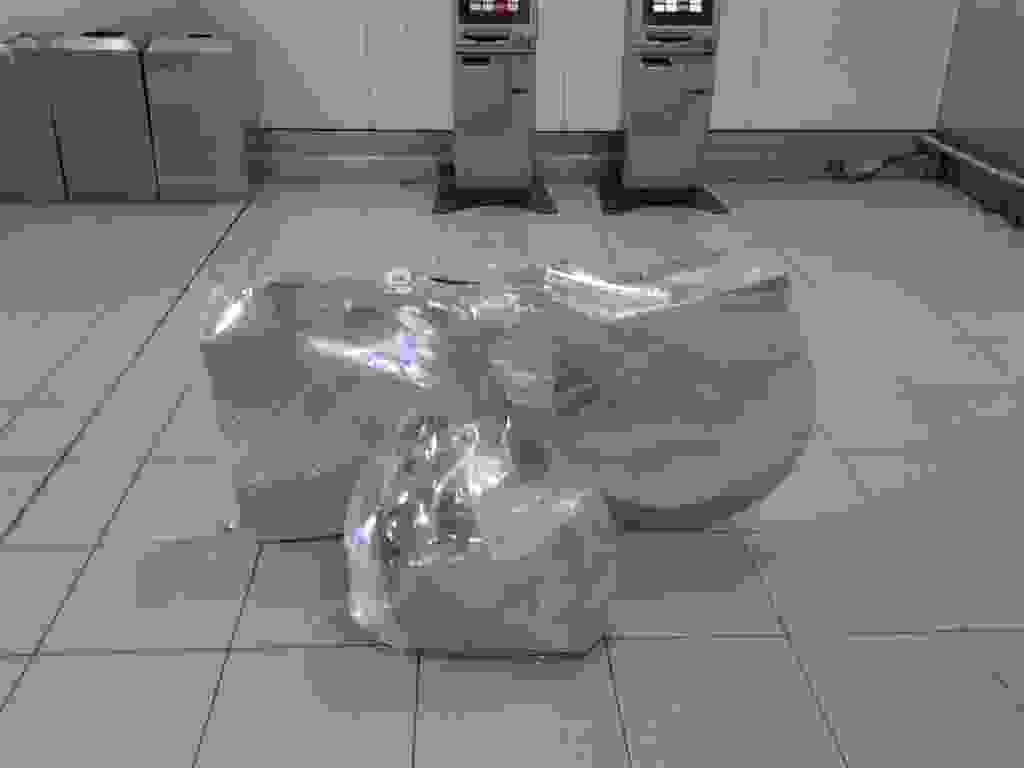
\includegraphics[width=\mywidth]{../wp-content/uploads/2015/07/20150711_182946-1024x768.jpg} \end{center}
\pagebreak

Arrivée à l'aéroport de Miami, les formalités sont très longues, vérification automatisée du passeport, puis manuelle, puis inspection des bagages avec la queue à chaque fois ! 
\begin{center} 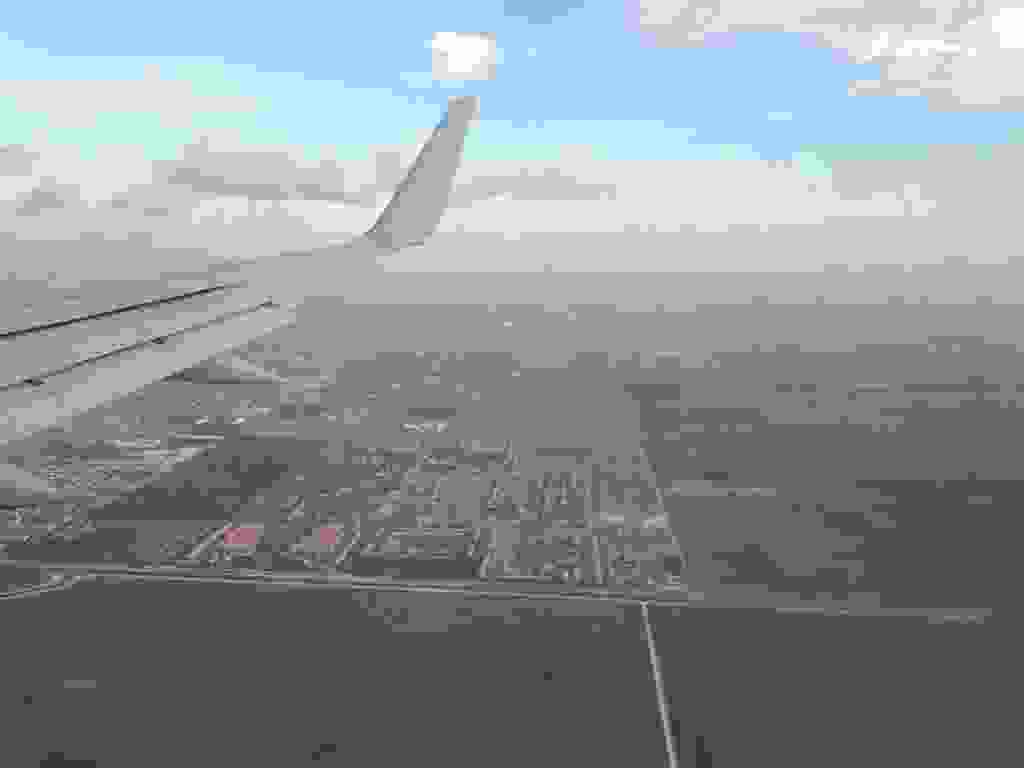
\includegraphics[width=\mywidth]{../wp-content/uploads/2015/07/20150712_005212-1024x768.jpg} \end{center}
\begin{center} 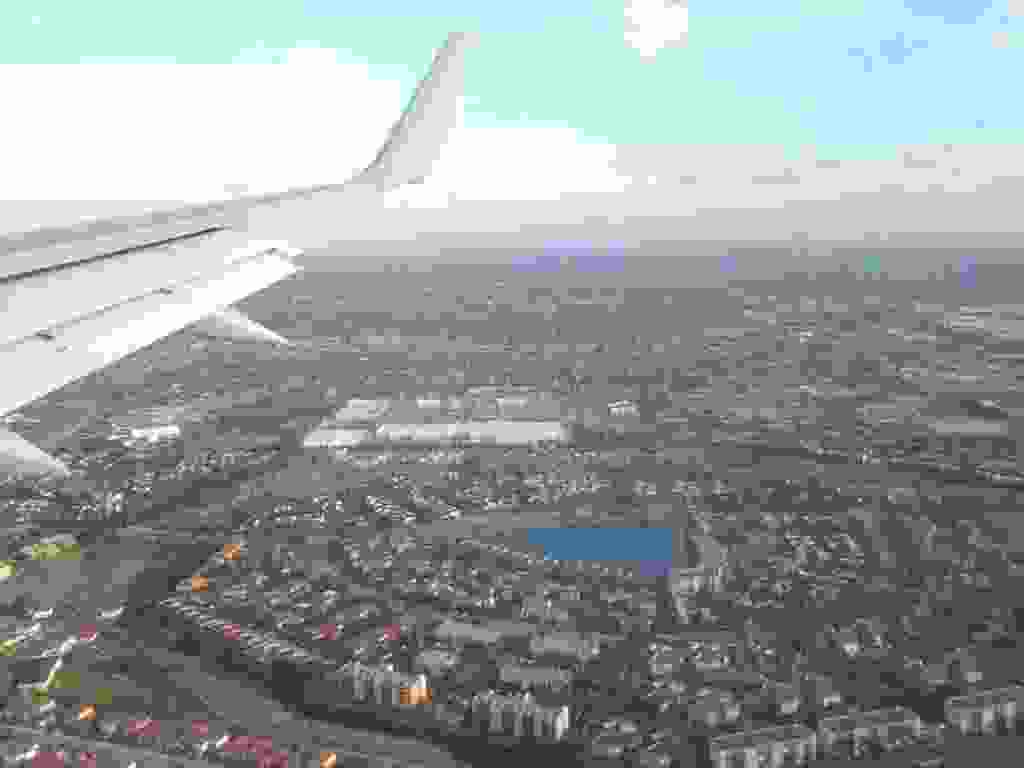
\includegraphics[width=\mywidth]{../wp-content/uploads/2015/07/20150712_005354-1024x768.jpg} \end{center}
\pagebreak

A Miami, Rane m'a hébergé dans la maison où il vit avec sa mère et 5 ou 6 autres colocataires, tous végétariens ou même vegan pour certains. 
\begin{center} 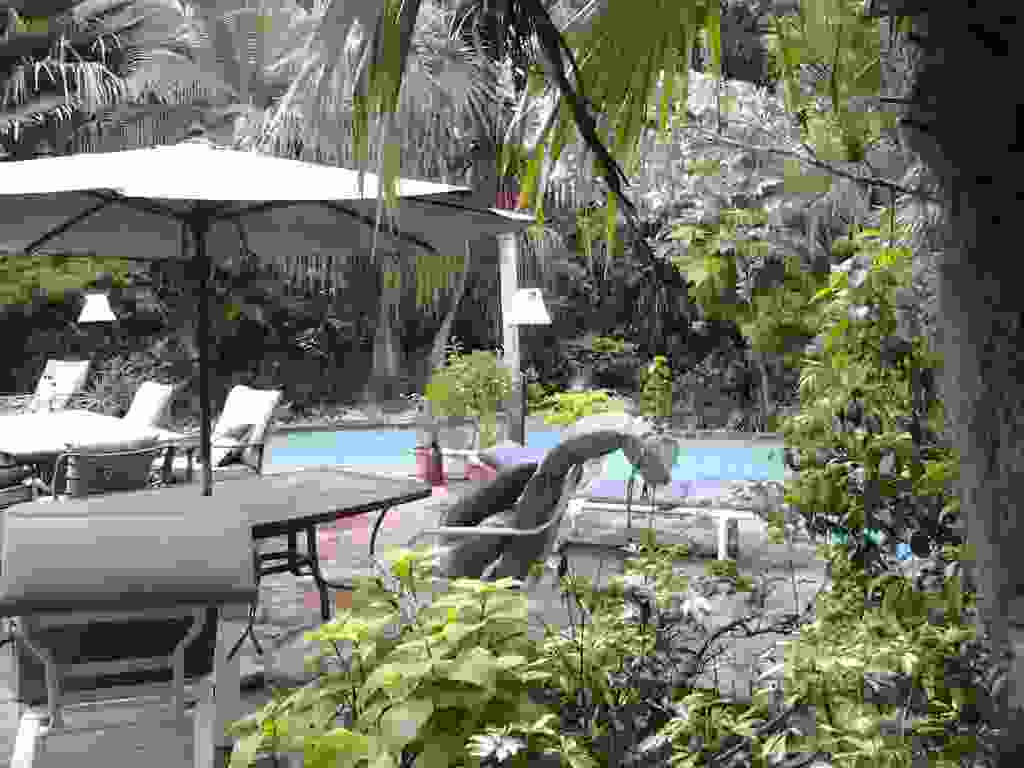
\includegraphics[width=\mywidth]{../wp-content/uploads/2015/07/20150714_222123-1024x768.jpg} \end{center}
\begin{center} 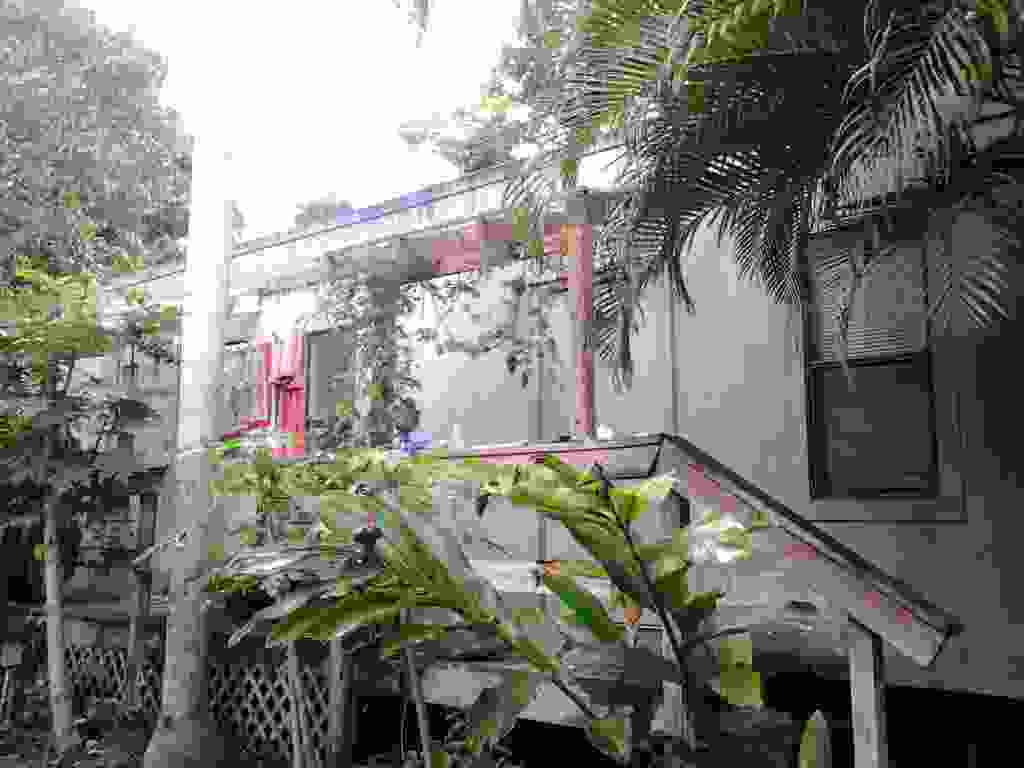
\includegraphics[width=\mywidth]{../wp-content/uploads/2015/07/20150714_222115-1024x768.jpg} \end{center}
\pagebreak

Le premier jour, je suis allé aider Rane à planter des patates douces sur le terrain de son père. 
\begin{center} 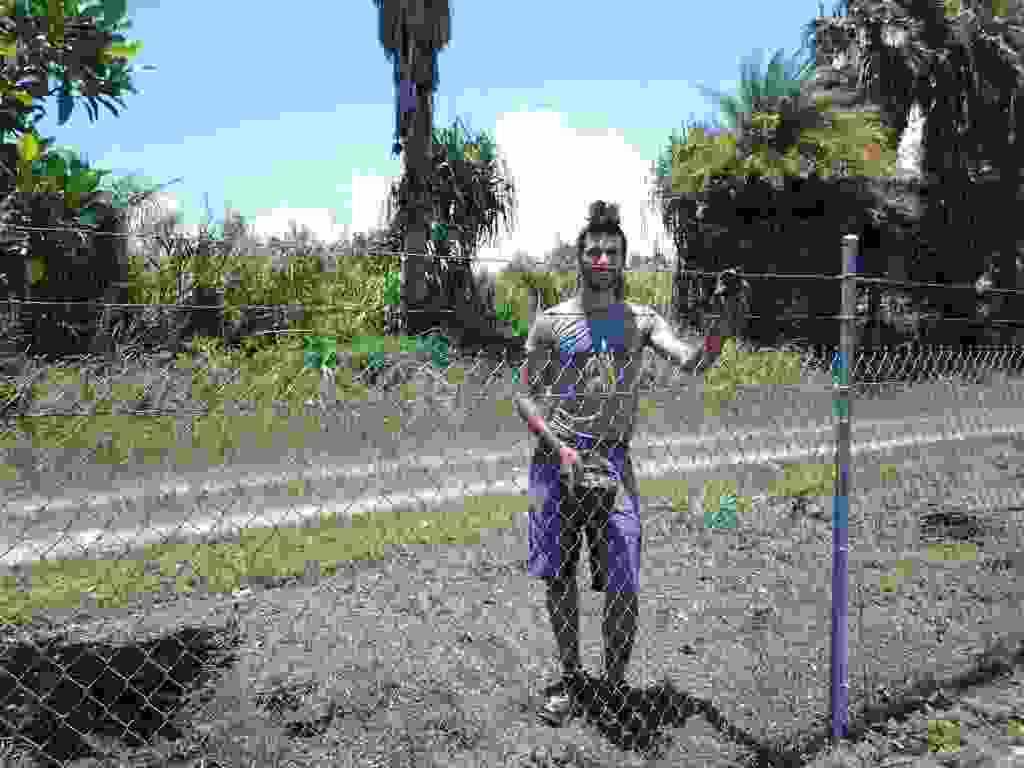
\includegraphics[width=\mywidth]{../wp-content/uploads/2015/07/20150712_184212-1024x768.jpg} \end{center}
\begin{center} 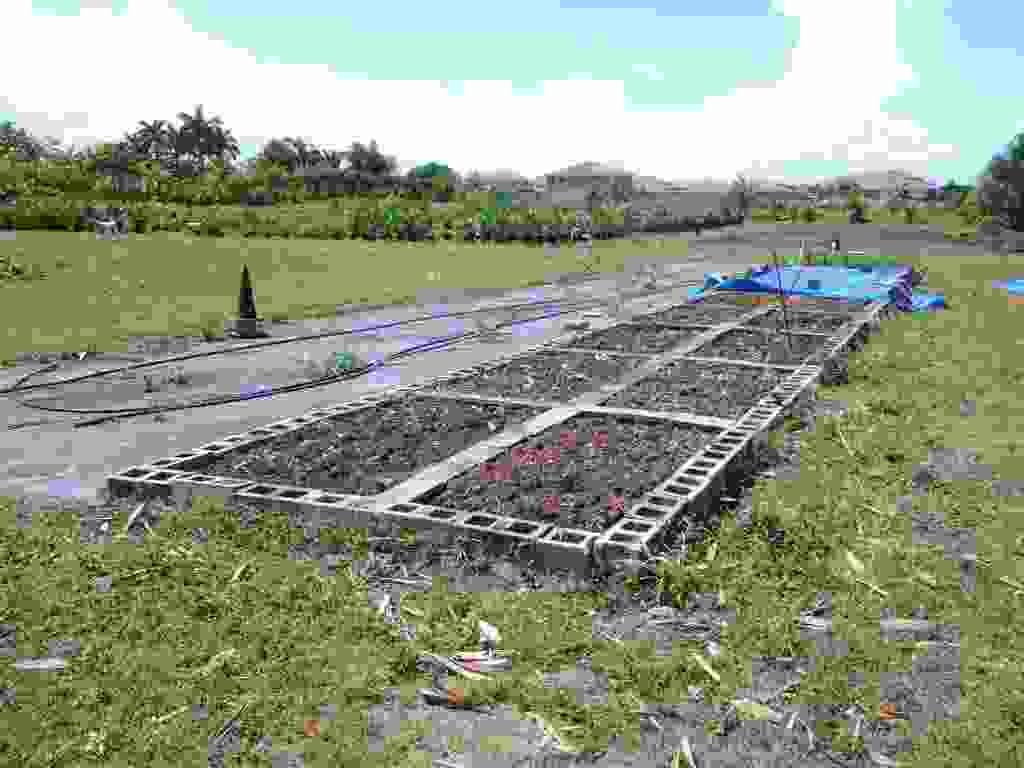
\includegraphics[width=\mywidth]{../wp-content/uploads/2015/07/20150712_212339-1024x768.jpg} \end{center}
\pagebreak

Repas chez le père de Rane avec la famille. 
\begin{center} 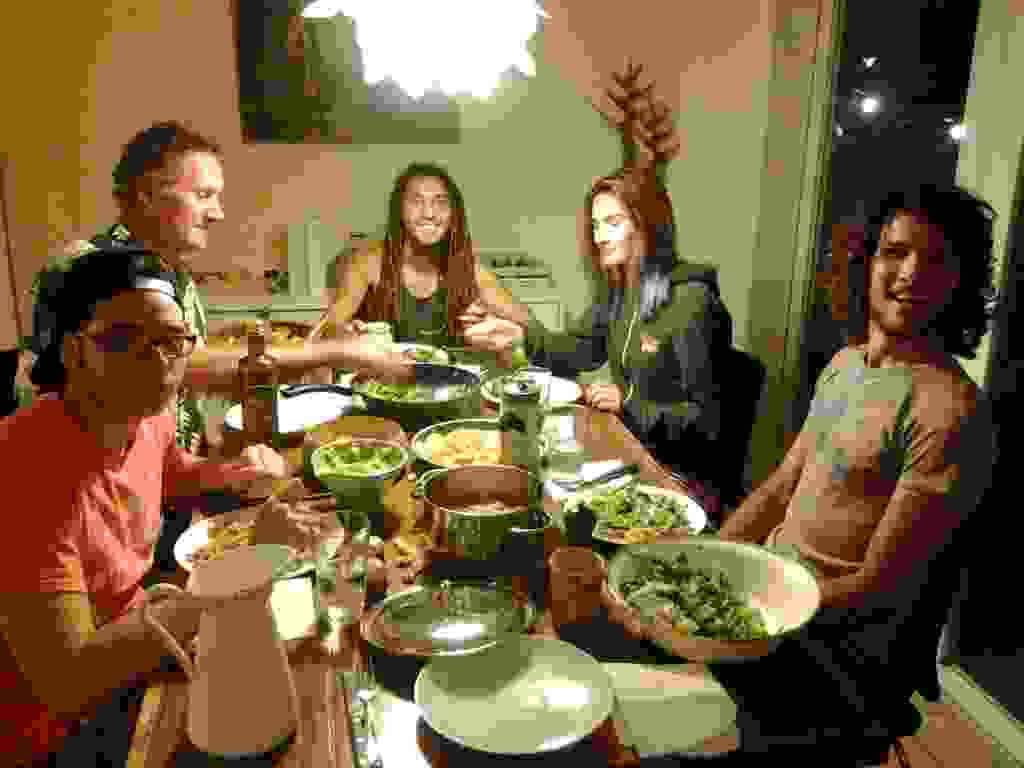
\includegraphics[width=\mywidth]{../wp-content/uploads/2015/07/20150713_031906-1024x768.jpg} \end{center}

Puis visite de Miami en vélo. 
\begin{center} 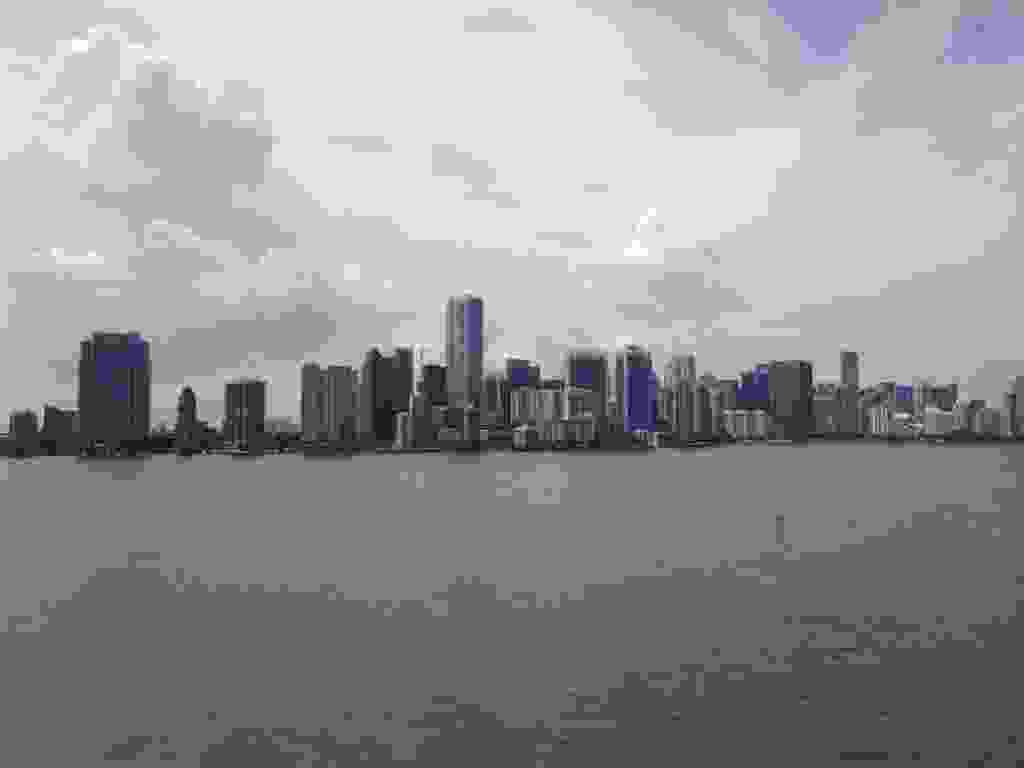
\includegraphics[width=\mywidth]{../wp-content/uploads/2015/07/20150713_205210-1024x768.jpg} \end{center}
\begin{center} 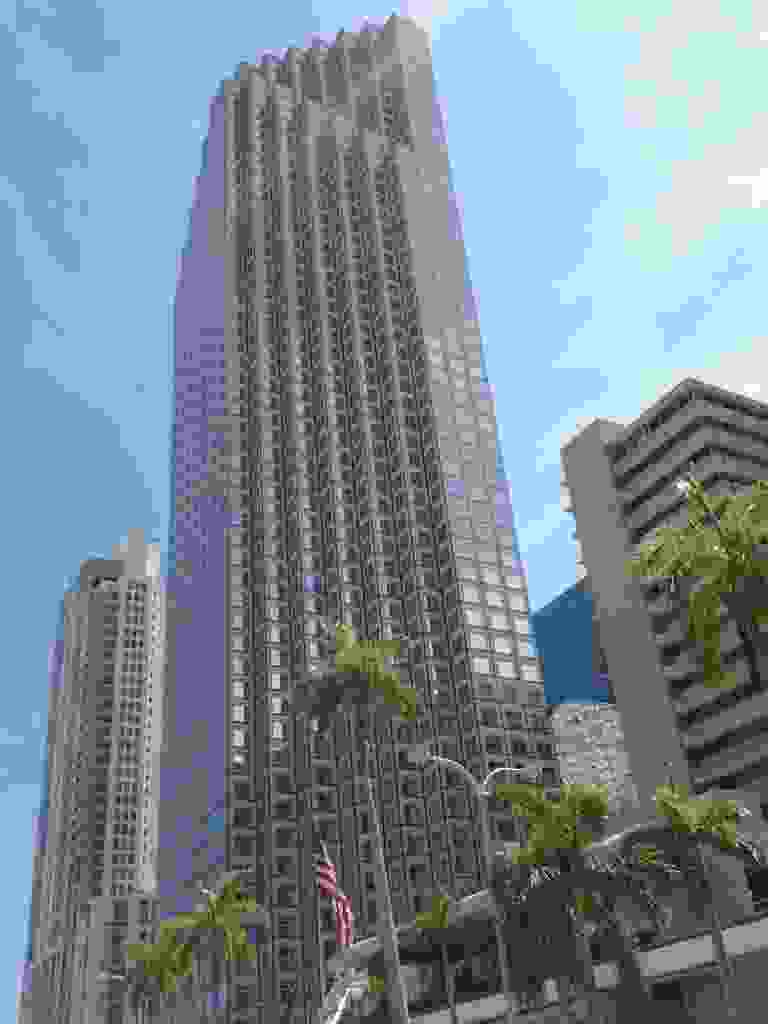
\includegraphics[width=\mywidth]{../wp-content/uploads/2015/07/20150713_211308-768x1024.jpg} \end{center}
\begin{center} 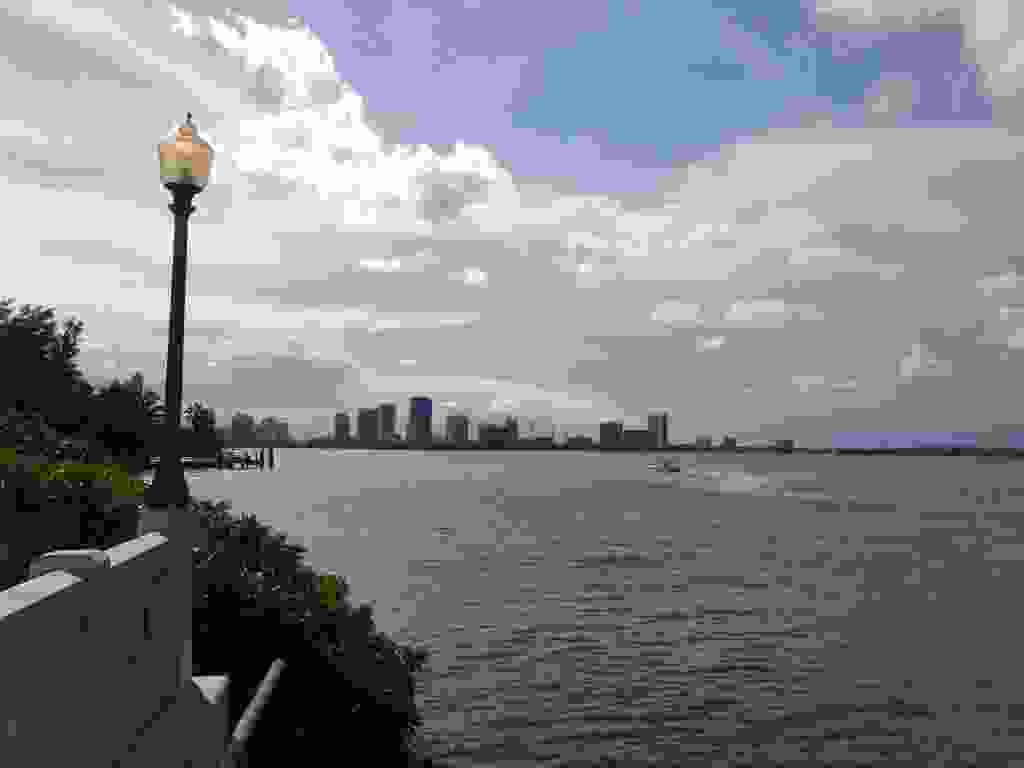
\includegraphics[width=\mywidth]{../wp-content/uploads/2015/07/20150713_230921-1024x768.jpg} \end{center}

Key Biscayne, une île au sud de Miami 
\begin{center} 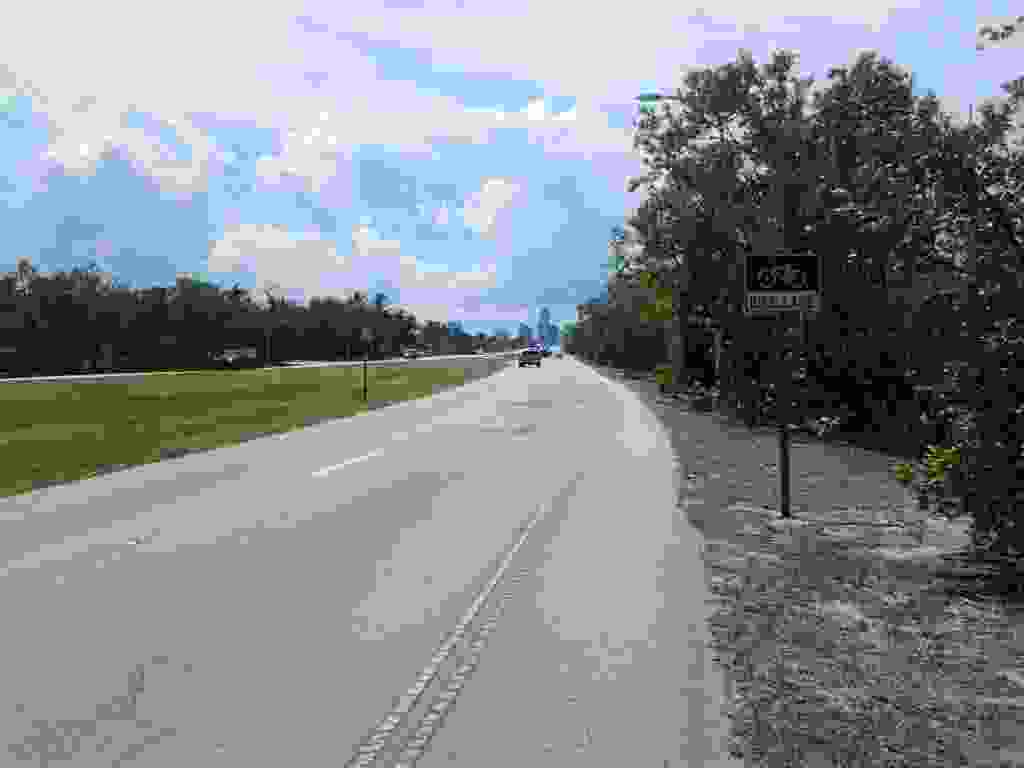
\includegraphics[width=\mywidth]{../wp-content/uploads/2015/07/20150713_204119-1024x768.jpg} \end{center}
\begin{center} 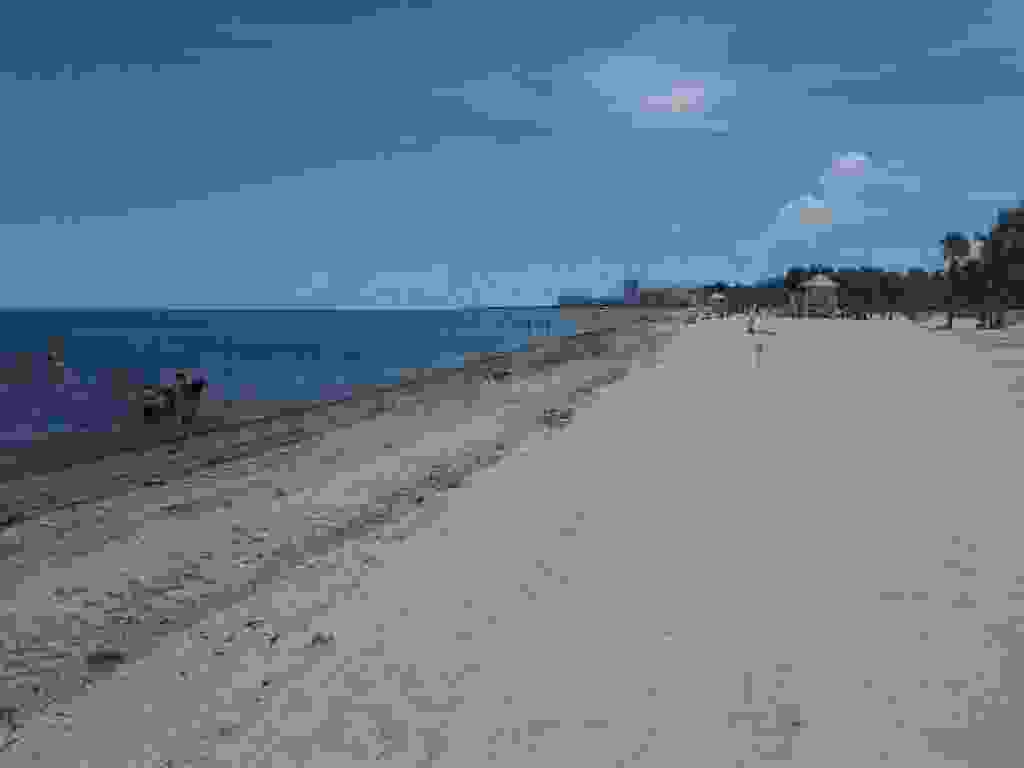
\includegraphics[width=\mywidth]{../wp-content/uploads/2015/07/20150713_202039-1024x768.jpg} \end{center}
\begin{center} 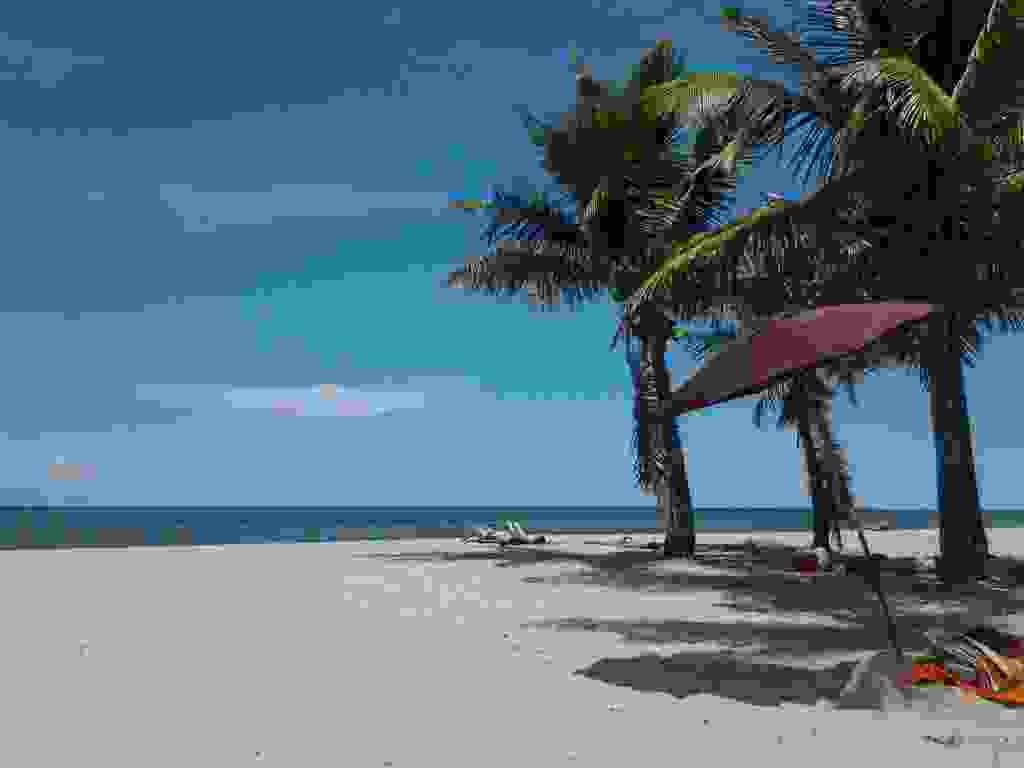
\includegraphics[width=\mywidth]{../wp-content/uploads/2015/07/20150713_202852-1024x768.jpg} \end{center}
\pagebreak

Miami Beach, un alignement de bars, hôtels et restaurants face à la mer. 
\begin{center} 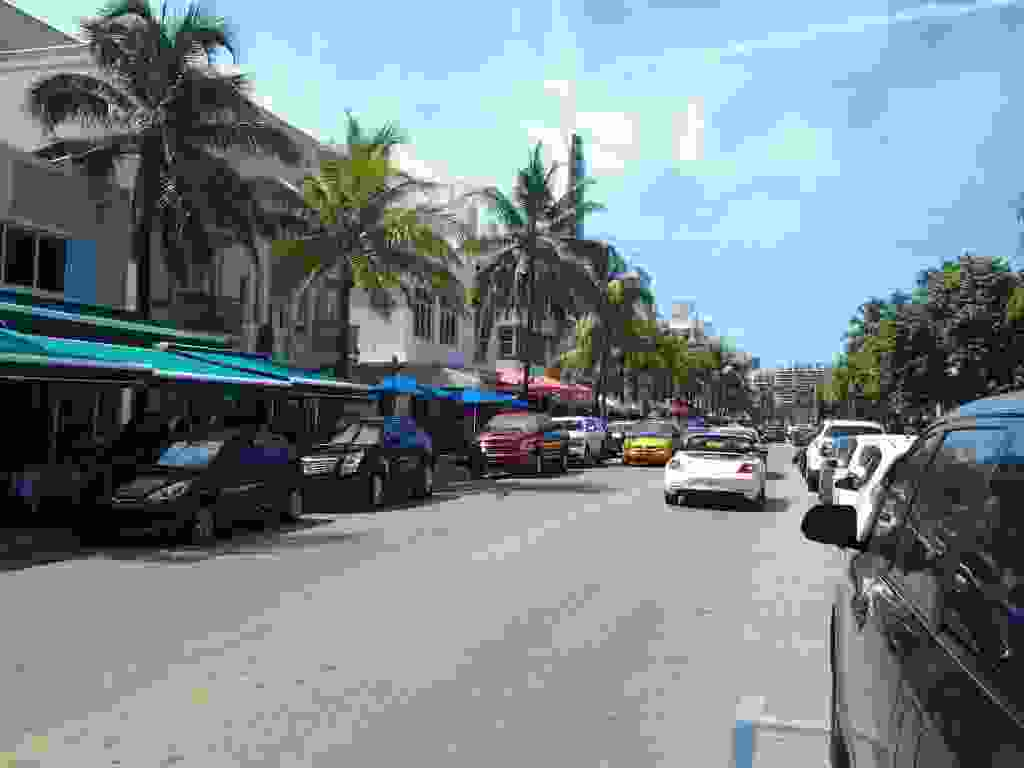
\includegraphics[width=\mywidth]{../wp-content/uploads/2015/07/20150713_214017-1024x768.jpg} \end{center}
\begin{center} 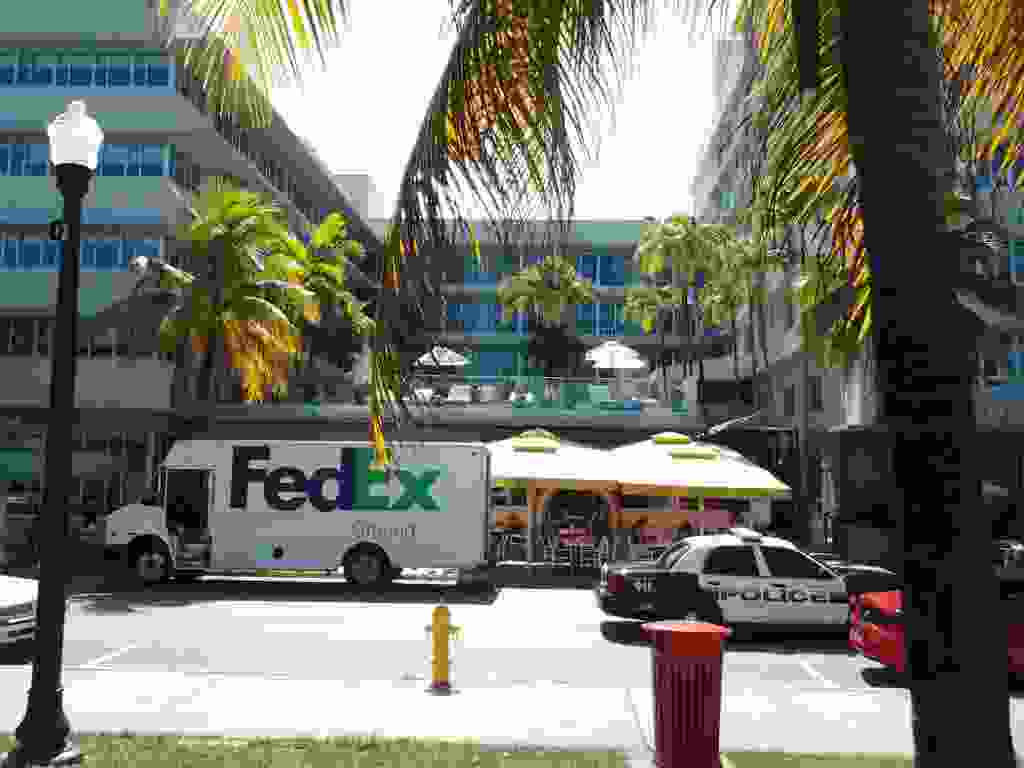
\includegraphics[width=\mywidth]{../wp-content/uploads/2015/07/20150713_220518-1024x768.jpg} \end{center}
\begin{center} 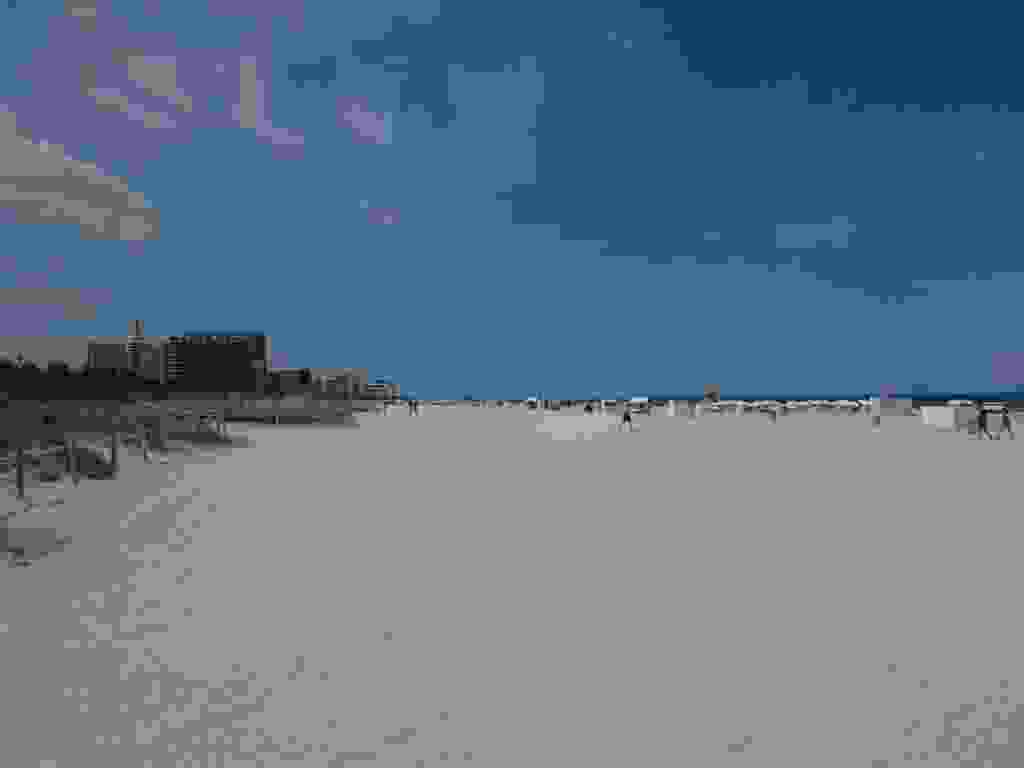
\includegraphics[width=\mywidth]{../wp-content/uploads/2015/07/20150713_214327-1024x768.jpg} \end{center}
\begin{center} 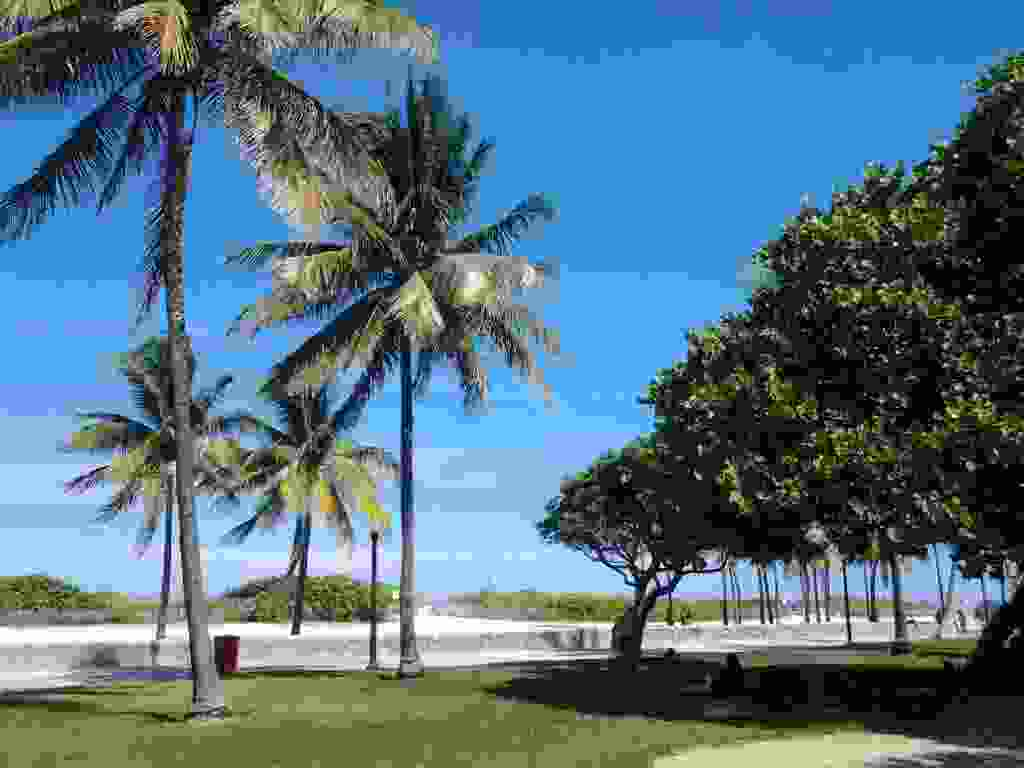
\includegraphics[width=\mywidth]{../wp-content/uploads/2015/07/20150713_220534-1024x768.jpg} \end{center}
